\documentclass[tikz,border=10pt]{standalone}
\usepackage{tikz}
\usetikzlibrary{positioning,arrows.meta,calc}

\begin{document}
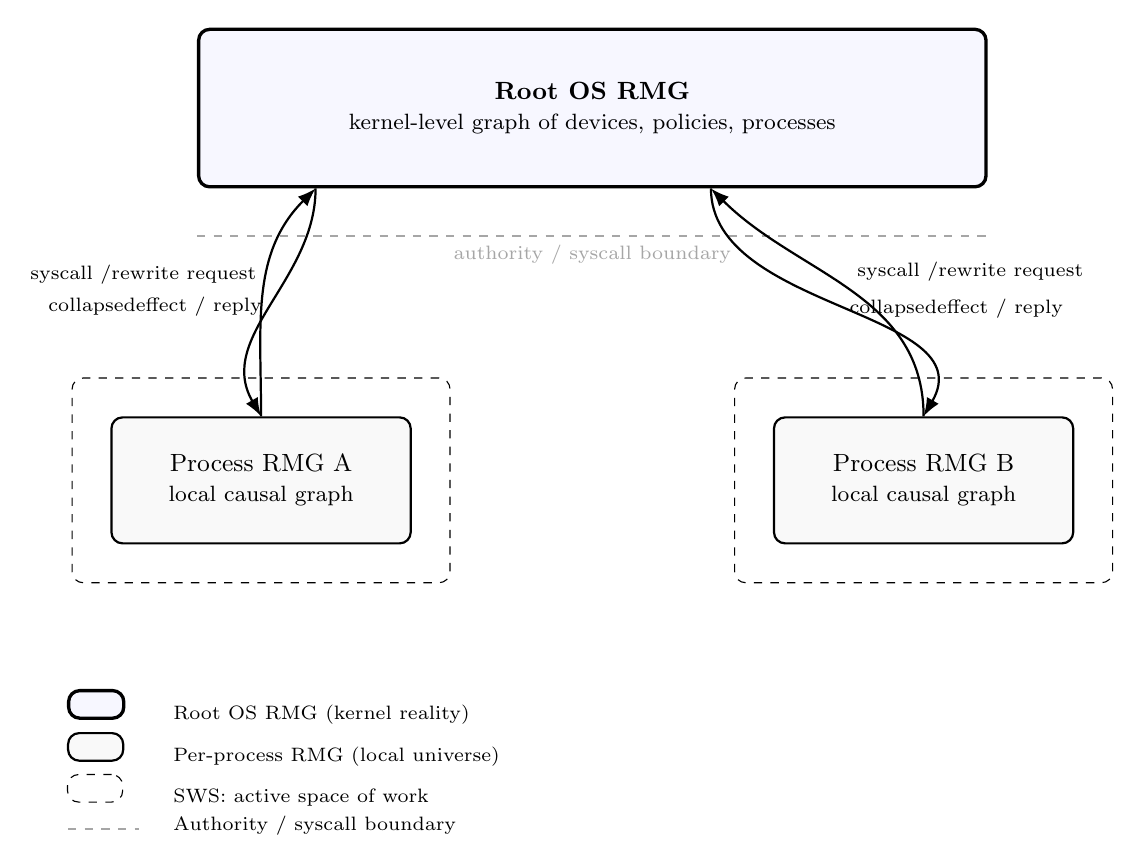
\begin{tikzpicture}[
  >=Latex,
  font=\small,
  rmg/.style={draw, rounded corners, thick, minimum width=3.8cm, minimum height=1.6cm, align=center, fill=gray!5},
  osrmg/.style={draw, rounded corners, very thick, minimum width=10cm, minimum height=2.0cm, align=center, fill=blue!3},
  sws/.style={draw, dashed, rounded corners, minimum width=4.8cm, minimum height=2.6cm, align=center},
  arrow/.style={->, thick},
  lbl/.style={font=\scriptsize, inner sep=1pt}
]

% Root OS RMG (kernel universe)
\node[osrmg] (os) {%
  \textbf{Root OS RMG}\\
  \footnotesize kernel-level graph of devices, policies, processes
};

% Authority / syscall boundary (logical line)
\draw[dashed, thick, gray!70] ($(os.south west)+(0,-0.6)$) -- ($(os.south east)+(0,-0.6)$)
  node[midway, below=2pt, lbl, fill=white] {authority / syscall boundary};

% SWS + Process RMG A
\node[sws, below left=2.4cm and 1.8cm of os.south] (swsA) {SWS A\\\footnotesize space of work state};
\node[rmg] at (swsA) (procA) {Process RMG A\\\footnotesize local causal graph};

% SWS + Process RMG B
\node[sws, below right=2.4cm and 1.8cm of os.south] (swsB) {SWS B\\\footnotesize space of work state};
\node[rmg] at (swsB) (procB) {Process RMG B\\\footnotesize local causal graph};

% Syscall / rewrite request arrows (up)
\draw[arrow] (procA.north) to[out=90,in=-135] node[lbl, above left=2pt] {%
  syscall /\\rewrite request
} ($(os.south west)!0.30!(os.south)$);

\draw[arrow] (procB.north) to[out=90,in=-45] node[lbl, above right=2pt] {%
  syscall /\\rewrite request
} ($(os.south east)!0.70!(os.south)$);

% Collapsed effect / response arrows (down)
\draw[arrow] ($(os.south west)!0.30!(os.south)$) to[out=-90,in=120]
  node[lbl, left=2pt] {collapsed\\effect / reply} (procA.north);

\draw[arrow] ($(os.south east)!0.70!(os.south)$) to[out=-90,in=60]
  node[lbl, right=2pt] {collapsed\\effect / reply} (procB.north);

% Legend (bottom)
\node[anchor=north west, lbl] at ($(swsA.south west)+(-0.1,-1.3)$) {%
  \begin{tabular}{@{}ll@{}}
    \tikz{\node[osrmg, minimum width=0.7cm, minimum height=0.35cm] {};}& Root OS RMG (kernel reality)\\[2pt]
    \tikz{\node[rmg, minimum width=0.7cm, minimum height=0.35cm] {};}& Per-process RMG (local universe)\\[2pt]
    \tikz{\node[sws, minimum width=0.7cm, minimum height=0.35cm] {};}& SWS: active space of work\\[2pt]
    \tikz{\draw[dashed, thick, gray!70] (0,0)--(0.9,0);}& Authority / syscall boundary
  \end{tabular}
};

\end{tikzpicture}
\end{document}